% Options for packages loaded elsewhere
\PassOptionsToPackage{unicode}{hyperref}
\PassOptionsToPackage{hyphens}{url}
%
\documentclass[
  ignorenonframetext,
  aspectratio=169]{beamer}
\usepackage{pgfpages}
\setbeamertemplate{caption}[numbered]
\setbeamertemplate{caption label separator}{: }
\setbeamercolor{caption name}{fg=normal text.fg}
\beamertemplatenavigationsymbolsempty
% Prevent slide breaks in the middle of a paragraph
\widowpenalties 1 10000
\raggedbottom
\setbeamertemplate{part page}{
  \centering
  \begin{beamercolorbox}[sep=16pt,center]{part title}
    \usebeamerfont{part title}\insertpart\par
  \end{beamercolorbox}
}
\setbeamertemplate{section page}{
  \centering
  \begin{beamercolorbox}[sep=12pt,center]{part title}
    \usebeamerfont{section title}\insertsection\par
  \end{beamercolorbox}
}
\setbeamertemplate{subsection page}{
  \centering
  \begin{beamercolorbox}[sep=8pt,center]{part title}
    \usebeamerfont{subsection title}\insertsubsection\par
  \end{beamercolorbox}
}
\AtBeginPart{
  \frame{\partpage}
}
\AtBeginSection{
  \ifbibliography
  \else
    \frame{\sectionpage}
  \fi
}
\AtBeginSubsection{
  \frame{\subsectionpage}
}
\usepackage{amsmath,amssymb}
\usepackage{lmodern}
\usepackage{iftex}
\ifPDFTeX
  \usepackage[T1]{fontenc}
  \usepackage[utf8]{inputenc}
  \usepackage{textcomp} % provide euro and other symbols
\else % if luatex or xetex
  \usepackage{unicode-math}
  \defaultfontfeatures{Scale=MatchLowercase}
  \defaultfontfeatures[\rmfamily]{Ligatures=TeX,Scale=1}
\fi
\usetheme[]{Dresden}
\usecolortheme{beaver}
\usefonttheme{structurebold}
% Use upquote if available, for straight quotes in verbatim environments
\IfFileExists{upquote.sty}{\usepackage{upquote}}{}
\IfFileExists{microtype.sty}{% use microtype if available
  \usepackage[]{microtype}
  \UseMicrotypeSet[protrusion]{basicmath} % disable protrusion for tt fonts
}{}
\makeatletter
\@ifundefined{KOMAClassName}{% if non-KOMA class
  \IfFileExists{parskip.sty}{%
    \usepackage{parskip}
  }{% else
    \setlength{\parindent}{0pt}
    \setlength{\parskip}{6pt plus 2pt minus 1pt}}
}{% if KOMA class
  \KOMAoptions{parskip=half}}
\makeatother
\usepackage{xcolor}
\IfFileExists{xurl.sty}{\usepackage{xurl}}{} % add URL line breaks if available
\IfFileExists{bookmark.sty}{\usepackage{bookmark}}{\usepackage{hyperref}}
\hypersetup{
  pdftitle={Financial Risk Management},
  pdfauthor={Jiahua (Java) Xu, Ph.D.},
  hidelinks,
  pdfcreator={LaTeX via pandoc}}
\urlstyle{same} % disable monospaced font for URLs
\newif\ifbibliography
\usepackage{longtable,booktabs,array}
\usepackage{calc} % for calculating minipage widths
\usepackage{caption}
% Make caption package work with longtable
\makeatletter
\def\fnum@table{\tablename~\thetable}
\makeatother
\usepackage{graphicx}
\makeatletter
\def\maxwidth{\ifdim\Gin@nat@width>\linewidth\linewidth\else\Gin@nat@width\fi}
\def\maxheight{\ifdim\Gin@nat@height>\textheight\textheight\else\Gin@nat@height\fi}
\makeatother
% Scale images if necessary, so that they will not overflow the page
% margins by default, and it is still possible to overwrite the defaults
% using explicit options in \includegraphics[width, height, ...]{}
\setkeys{Gin}{width=\maxwidth,height=\maxheight,keepaspectratio}
% Set default figure placement to htbp
\makeatletter
\def\fps@figure{htbp}
\makeatother
\setlength{\emergencystretch}{3em} % prevent overfull lines
\providecommand{\tightlist}{%
  \setlength{\itemsep}{0pt}\setlength{\parskip}{0pt}}
\setcounter{secnumdepth}{-\maxdimen} % remove section numbering
\usepackage{tabularx,ragged2e,booktabs,rotating,pdflscape,xcolor,colortbl,tikz}
\usepackage{algorithm}
\usepackage{algorithmic}
\usepackage[justification=centering]{caption}

\hypersetup{colorlinks,linkcolor={blue},citecolor={black},urlcolor={blue}}

\setbeamertemplate{headline}{}

\setbeamertemplate{navigation symbols}[horizontal]

\setbeamertemplate{footline}
{
    \leavevmode
    \hbox{
        \begin{beamercolorbox}[wd=.2\paperwidth,ht=2.25ex,dp=2ex,center]{author in head/foot}\insertshortauthor
        \end{beamercolorbox}
        \begin{beamercolorbox}[wd=.6\paperwidth,ht=2.25ex,dp=2ex,center]{title in head/foot}\inserttitle
        \end{beamercolorbox}
        \begin{beamercolorbox}[wd=.2\paperwidth,ht=2.25ex,dp=2ex,center]{date in head/foot}\insertframenumber{} / \inserttotalframenumber
        \end{beamercolorbox}
        }
        \vskip0pt
    }

% \titlegraphic{
% \includegraphics[width=3cm,height=3cm,keepaspectratio]{figure/edheclogo}
% }


\beamertemplatenavigationsymbolsempty


% The following allows multi-columns

\newenvironment{cols}[1][]{}{}

\newenvironment{col}[1]{\begin{minipage}{#1}\ignorespaces}{%
\end{minipage}
\ifhmode\unskip\fi
\aftergroup\useignorespacesandallpars}

\def\useignorespacesandallpars#1\ignorespaces\fi{%
#1\fi\ignorespacesandallpars}

\makeatletter
\def\ignorespacesandallpars{%
  \@ifnextchar\par
    {\expandafter\ignorespacesandallpars\@gobble}%
    {}%
}
\makeatother
\ifLuaTeX
  \usepackage{selnolig}  % disable illegal ligatures
\fi

\title{Financial Risk Management}
\subtitle{Derivatives}
\author{Jiahua (Java) Xu, Ph.D.}
\date{2022}

\begin{document}
\frame{\titlepage}

\begin{frame}{What are derivatives}
\protect\hypertarget{what-are-derivatives}{}
A derivative is

\begin{itemize}
\tightlist
\item
  a financial security or contract whose value \textbf{derives} from the
  value of another asset / assets, known as the \textbf{underlying} (UL)
\item
  an instrument for \textbf{transferring risk} and can therefore be used
  for

  \begin{itemize}
  \tightlist
  \item
    \textbf{hedging}: alter the exposure to an asset / risk you already
    have
  \item
    \textbf{investment / speculation}: take on an exposure to an asset /
    risk
  \end{itemize}
\end{itemize}
\end{frame}

\begin{frame}{Forward}
\protect\hypertarget{forward}{}
A forward is

\begin{itemize}
\tightlist
\item
  an OTC (over-the-counter) contract in which two counterparties agree,
  with zero money down, to buy / sell the UCL at a pre-agreed
  \emph{forward price} at a given \emph{delivery date} in the future
\end{itemize}

The contract is an \emph{obligation} of both parties to transact,
designed to protect both the buyer and the seller from price
fluctuations in the future.
\end{frame}

\begin{frame}{Investment assets and consumption assets}
\protect\hypertarget{investment-assets-and-consumption-assets}{}
\textbf{Investment asset}: asset normally held for investment purposes

\begin{itemize}
\tightlist
\item
  financial assets: stocks, bonds
\item
  precious metal: gold, silver
\end{itemize}

\textbf{consumption asset}: asset NOT normally held for investment
purposes

\begin{itemize}
\tightlist
\item
  industrial metals: copper, aluminium
\item
  agricultural products: orange juice, pork bellies
\item
  energy products: natural gas, heating oil
\end{itemize}
\end{frame}

\begin{frame}
\begin{block}{Example}
\protect\hypertarget{example}{}
a forward contract to exchange 1m barrels of crude oil in 3 months at a
forward price of USD 95/barrel

At the \emph{delivery date}:

\begin{itemize}
\tightlist
\item
  The buyer (Long) delivers: forward price USD 95m
\item
  The seller (Short) delivers: UL 1m barrels of crude oil
\end{itemize}
\end{block}
\end{frame}

\begin{frame}{Payoff of a forward}
\protect\hypertarget{payoff-of-a-forward}{}
\begin{block}{Notations}
\protect\hypertarget{notations}{}
\(F\): forward price

\(T\): delivery date

\(S_T\): the spot price of the underlying on the delivery date
\end{block}

\begin{block}{Payoff diagrams}
\protect\hypertarget{payoff-diagrams}{}
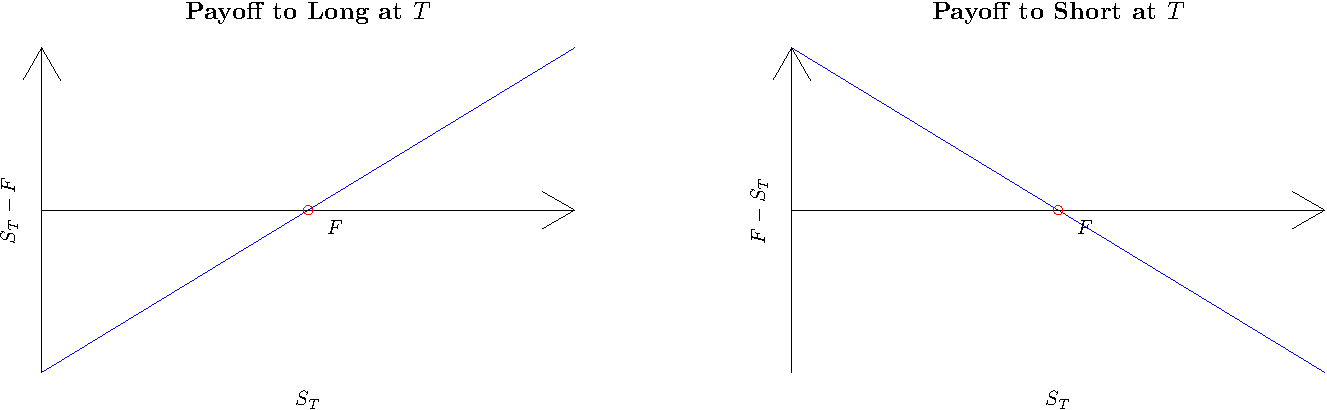
\includegraphics{figure/unnamed-chunk-5-1.pdf}
\end{block}
\end{frame}

\begin{frame}{Fair forward price}
\protect\hypertarget{fair-forward-price}{}
\begin{itemize}
\item
  Consider a stock

  \begin{itemize}
  \tightlist
  \item
    currently traded at £40
  \item
    does not pay dividends
  \item
    with an expected return of 5\% p.a.
  \item
    risk-free rate is 2\% p.a.
  \end{itemize}
\item
  How much would you \textbf{agree to} today, to pay to buy the stock a
  year from now?
\end{itemize}

\begin{enumerate}
[(a)]
\tightlist
\item
  £40
\item
  £40.8
\item
  £42
\end{enumerate}
\end{frame}

\begin{frame}{Arbitrage-free pricing}
\protect\hypertarget{arbitrage-free-pricing}{}
Replicate the same cashflow as a long forward contract by buying the
stock today using borrowed money and repaying the borrowing with
interest at \(T\):

\begin{longtable}[]{@{}lll@{}}
\toprule
& Today & \textbf{Delivery date} \(T\) \\
\midrule
\endhead
\textbf{Long forward} & 0 & \(S_T-F\) \\
``Cash and carry'' replicating strategy: & & \\
Buy stock today & \(-40\) & \(S_T\) \\
Borrow £40 for 1 year at 2\% & \(40\) & \(-40.8\) \\
\textbf{Net} & 0 & \(S_T-40.8\) \\
\bottomrule
\end{longtable}
\end{frame}

\begin{frame}
The fair forward price is 40.8; otherwise there is an arbitrage
opportunity.

For example, if the actual forward price is quoted at 41.2

\begin{longtable}[]{@{}llll@{}}
\toprule
& & Today & \textbf{Delivery date} \(T\) \\
\midrule
\endhead
\textbf{Buy low:} & Buy stock today & \(-40\) & \(S_T\) \\
& Borrow £40 for 1 year at 2\% & 40 & \(-40.8\) \\
& Net & 0 & \(S_T-40.8\) \\
& & & \\
\textbf{Sell high:} & Short forward & 0 & \(41.2-S_T\) \\
& & & \\
\textbf{Net cash flows} & & 0 & £0.4 \\
\bottomrule
\end{longtable}
\end{frame}

\begin{frame}{Cost of carry relationship}
\protect\hypertarget{cost-of-carry-relationship}{}
\begin{itemize}
\item
  Consider another stock

  \begin{itemize}
  \tightlist
  \item
    currently traded at £40
  \item
    pays a dividend of £1 in 5 months
  \item
    with an expected return of 5\% p.a.
  \item
    risk-free rate is 2\% p.a.
  \end{itemize}
\item
  How much would you \textbf{agree to} today, to pay to buy the stock a
  year from now?
\end{itemize}

\(40 \times (1+2\%) - 1 \times (1+2\% \times \frac{6}{12}) = 39.79\)
\end{frame}

\begin{frame}
For assets that can be traded spot and stored, forwards futures prices
are linked to spot prices through the ``cost of carry'' relationship:

\[
F = S \times (1+r_j)^T - FV(\text{holding benefits}) + FV(\text{holding costs})
\] where

\(F\): forward price

\(S\): current spot price

\(r_f\): risk-free rate

\(T\): maturity of the contract

Holding benefits (costs) are the benefits (costs), typically cashflows,
associated with holding the UL that you miss when buying in the future
compared to buying now

\(FV\): future value, i.e.~compounded to \(T\) at risk-free rate
\end{frame}

\begin{frame}{Futures}
\protect\hypertarget{futures}{}
\textbf{Future contract}: fungible, standardized contract for delivery
of a specific commodity at a specific delivery or maturity date for an
agreed-upon price (the \textbf{futures price}), to be paid at contract
maturity

\textbf{Future market}: market for trading \textbf{futures contracts}
wherein buyers and sellers in a centralized futures exchange (wherein
some flexibility is sacrificed for \textbf{liquidity})
\end{frame}

\begin{frame}
The \textbf{futures exchange} establishes features of the contract:

\begin{itemize}
\tightlist
\item
  \textbf{size} of the contract: mass, volume, number of units
\item
  acceptable \textbf{grade} of the commodity
\item
  contract \textbf{delivery dates}
\item
  nature of \textbf{settlement}: cash, warehouse receipts
\end{itemize}

The trader with the \textbf{long position} (the buyer) commits to
purchasing the commodity on the delivery date.

The trader with the \textbf{short position} (the seller) delivering the
commodity on the delivery date.
\end{frame}

\begin{frame}{Forwards vs Futures}
\protect\hypertarget{forwards-vs-futures}{}
Futures are \textbf{exchange-traded} version of forwards

\begin{longtable}[]{@{}lll@{}}
\toprule
& \textbf{Forwards} & \textbf{Futures} \\
\midrule
\endhead
Buyer-seller interaction & Direct & Via exchange \\
Default-risk borne by & Individual parties & Exchange \\
Default controlled by & Collateral & Margin accounts daily ``marking to
market'' \\
Contract terms & Tailored & Standardized \\
Unilateral reversal & Difficult & Easy \\
\bottomrule
\end{longtable}
\end{frame}

\begin{frame}{E-mini S\&P500 Index Futures Contract}
\protect\hypertarget{e-mini-sp500-index-futures-contract}{}
Most popular equity index futures contract in the world

\begin{itemize}
\tightlist
\item
  \textbf{Contract size}: \$50 \(\times\) S\&P500 Index price (0.2 of
  the standard S\&P500 futures contract)
\item
  \textbf{Contract month}: March quarterly expiration cycle (Mar, Jun,
  Sep, Dec)
\item
  \textbf{Trading hours}: CME Globex (essentially around the clock from
  Sunday evening to late Friday afternoon)
\item
  \textbf{Trading termination}: 8.30am on the Settlement Date (3rd
  Friday of the contract month)
\item
  \textbf{Settlement procedure}: Cash settlement based on the Special
  Opening Quotation on Friday morning of the S\&P500 Index
\item
  \textbf{Position limits}: 20,000 S\&P500 contracts or equivalent net
  long or short in all contract months combined
\end{itemize}
\end{frame}

\begin{frame}{Futures contracts - marking to market}
\protect\hypertarget{futures-contracts---marking-to-market}{}
\begin{itemize}
\item
  Similar economic effect to forwards, but, due to \textbf{marking to
  market}, gains and losses on futures positions are settled each day
\item
  After \textbf{marking to market}, both sides have a zero value
  position with the new (end of day) futures price.
\item
  The long receives from (pays to) the short any increase (decrease) in
  the futures price from the previous day
\end{itemize}

\begin{longtable}[]{@{}llllll@{}}
\toprule
Date & 0 & 1 & 2 & 3 & \(T=4\) \\
\midrule
\endhead
Future price & 106 & 108 & 104 & 105 & \(S_T=107\) \\
Long receives & 0 & 108-106=2 & 104-108=-4 & 105-104=1 & 107-105=2 \\
\bottomrule
\end{longtable}

\begin{itemize}
\tightlist
\item
  Note that \(\sum(\text{cash flow long receives}) = 1\), equal to the
  payoff on a forward position where the forward price is the original
  futures price \(S_T - F = 107-106 = 1\)
\item
  \textbf{Convergence property}: at maturity, the futures price and spot
  price must converge; \(F_T=P_T\)
\end{itemize}
\end{frame}

\begin{frame}{The clearinghouse}
\protect\hypertarget{the-clearinghouse}{}
\textbf{Clearinghouse}: designated intermediary between a buyer and a
seller in a financial market that validates and finalizes the
transaction, ensuring that both the buyer and the seller honour their
contractual obligations.

\begin{itemize}
\tightlist
\item
  Traders on both sides face the \textbf{clearinghouse} rather than each
  other.
\item
  The \textbf{clearinghouse} bears the risk of non-performance by any
  trader.
\item
  Contracts are therefore \textbf{fungible}: traders can reverse a
  position by entering the countervailing position with the
  clearinghouse.
\end{itemize}
\end{frame}

\begin{frame}{Margin and open interest}
\protect\hypertarget{margin-and-open-interest}{}
\textbf{Margin}: a good-faith deposit to guarantee contract performance

\textbf{Marking to market}: daily settling (realizing) of gains and
losses with the clearinghouse {[}note special tax treatment{]}

\textbf{Maintenance margin}: minimum quantity that a trader must hold in
reserve with the clearinghouse

\begin{itemize}
\tightlist
\item
  Margin safeguards the position of the clearninghouse.
\item
  If the mark-to-market value of the trader's account falls below the
  maintenance margin, the trader receives a \textbf{margin call}.
\item
  A \textbf{margin call} requires the trader to replenish the margin
  account to the maintenance margin. Otherwise, the position is reduced
  to a size commensurate with the remaining funds (the trader is
  \textbf{bought in} by the exchange).
\end{itemize}

\textbf{Open interest}: the number of contracts outstanding

\begin{itemize}
\tightlist
\item
  The position of the clearinghouse always nets out to zero.
\end{itemize}
\end{frame}

\begin{frame}{Hedging and speculation}
\protect\hypertarget{hedging-and-speculation}{}
\textbf{Hedgers} use futures to insulate themselves (\textbf{hedge})
against price movements in the underlying asset.

\begin{itemize}
\tightlist
\item
  Example: both airplane manufacturers and bauxite miners might seek to
  hedge their exposure to the price of aluminium.
\end{itemize}

\textbf{Speculators} use futures to profit from movements in futures
prices.

\begin{itemize}
\tightlist
\item
  Speculators take \textbf{long} position if they expect an increase in
  price and a \textbf{short} position if they expect a decrease in
  price.
\item
  Usually, \textbf{transaction costs} in future markets are considerably
  smaller than in markets for the UL.
\item
  Speculators also gain the advantage of \textbf{leverage} because
  margin requirements are generally much less than the value of the UL.
\end{itemize}
\end{frame}

\begin{frame}{Forward and future -- applications}
\protect\hypertarget{forward-and-future-applications}{}
\begin{itemize}
\tightlist
\item
  Contracts for difference (CFDs)
\item
  Profitable alpha (futures overlay) strategies
\item
  Commodities investing
\end{itemize}
\end{frame}

\begin{frame}{Contracts for difference (CFDs)}
\protect\hypertarget{contracts-for-difference-cfds}{}
A CFD is a contract between a buyer and a seller, stipulating that:

\begin{itemize}
\tightlist
\item
  if the price of the UL increases, the seller pays the buyer the
  increase
\item
  if the price falls, the buyer pays the seller the decrease
\end{itemize}

\begin{longtable}[]{@{}lll@{}}
\toprule
Cashflows & Today & \(T\) \\
\midrule
\endhead
to CFD buyer (long) & 0 & \(S_T-S\) \\
to CFD seller (short) & 0 & \(S-S_T\) \\
\bottomrule
\end{longtable}

In addition:

\begin{itemize}
\tightlist
\item
  the buyer pays the seller daily interst on the initial value of the UL
\item
  the seller pays the buyer any dividends / coupons on the underlying
\item
  margin requirements for end user
\end{itemize}
\end{frame}

\begin{frame}{CFDs vs forwards \& futures}
\protect\hypertarget{cfds-vs-forwards-futures}{}
\begin{longtable}[]{@{}llll@{}}
\toprule
Cashflows & Today & From today to \(T\) & \(T\) \\
\midrule
\endhead
to CFD buyer (long) & 0 & interest on \(S\) & \(S_T-S\) \\
to CFD seller (short) & 0 & 0 & \(S-S_T\) \\
\bottomrule
\end{longtable}
\end{frame}

\begin{frame}{Is the forward price the expected spot price?}
\protect\hypertarget{is-the-forward-price-the-expected-spot-price}{}
\begin{itemize}
\tightlist
\item
  is \(F=\mathbb{E}[S_T]\)
\item
  Simplest setting: ignoring holding costs / benefits, using simple
  compounding at an annual risk-free rate \(r_f\), for a 1-year forward
\end{itemize}

\[F = S \times (1+r_f)\]

\begin{itemize}
\tightlist
\item
  According to standard finance theories, the (risky) UL should earn a
  risk premium \(\pi\)
\end{itemize}

\(\mathbb{E}[S_T] = S \times (1+r_f+\pi)\)

therefore \(F \neq \mathbb{E}[S_T]\)
\end{frame}

\begin{frame}
\begin{itemize}
\item
  Actual payoff on a long forward: \(S_T - F\)
\item
  The \textbf{expected} payoff on a long forward is \[
  \mathbb{E}[S_T-F] = S \times (1 + r_f + \pi) - S \times (1 + r_f) = S \times \pi
  \]
\item
  The expected return on the long forward (as a percentage of the
  \emph{current price of the underlying}) is the risk premium
\item
  By going long (short) forwards / futures you assume (lay off) the risk
  premium on the UL
\end{itemize}
\end{frame}

\begin{frame}{Portable alpha strategies}
\protect\hypertarget{portable-alpha-strategies}{}
\begin{itemize}
\tightlist
\item
  According to the CAPM, the risk premium on a stokc or portfolio is:
\end{itemize}

\(\mathbb{E}(R_i) - R_f = \beta[\mathbb{E}(R_m) - R_f]\) where
\(\beta = \frac{\sigma_{R_i,R_m}}{\sigma^2_{R_m}}\)

where:

\(R_i,R_m\): the returns on the portfolio and the ``market'',
respectively

\(R_f\): the risk-free rate of return

\(\mathbb{E}[]\): expected value

\(\sigma_{R_i,R_m}\): the covariance between \(R_i\) and \(R_m\)

\(\sigma^2_{R_m}\): the variance of \(R_m\)

\begin{itemize}
\tightlist
\item
  The expected excess return on a stock is compensation for taking on
  (non-diversifiable) ``market'' risk
\end{itemize}
\end{frame}

\begin{frame}
If you run the regression:

\[
R_i - R_f = \alpha + \beta (R_m - R_f)  + \epsilon
\]

and securities are efficiently priced, alpha should not be statistically
significantly different from zero

\begin{itemize}
\tightlist
\item
  For actively managed portfolios, if alpha is positive this is
  typically interpreted as evidence of stock-picking ability
\end{itemize}
\end{frame}

\begin{frame}
Use futures overlays to create a position where you earn beta in one
asset category and alpha in another:

\begin{itemize}
\tightlist
\item
  You have £1m to invest and a target beta of 1 wrt the S\&P500
\item
  You believe there are no alpha opportunities in S\&P500 stocks but you
  have identified a market-neutral (zero-beta) hedge fund that you
  believe will generate positive alpha
\end{itemize}

To capture the S\&P beta return as well as the hedge fund alpha:

\begin{itemize}
\tightlist
\item
  invest £1m in the ``market-neutral'' hedge fund
\item
  go long £1m 1-yr S\&P500 futures
\end{itemize}
\end{frame}

\begin{frame}{Commodity forwards / futures pricing}
\protect\hypertarget{commodity-forwards-futures-pricing}{}
\begin{itemize}
\tightlist
\item
  The cost of carry relationship
\end{itemize}

\(F = S + \text{intest cost} - \text{holding benefit} + \text{holding costs}\)

\begin{itemize}
\tightlist
\item
  For commodities, this becomes
\end{itemize}

\(F = S + \text{intest cost} - \text{convenience yield} + \text{storage costs}\)

Convenience yield

\begin{itemize}
\tightlist
\item
  The convenicen yield (CY) is a holding benefit
\item
  Unlike holding benefits on financial aseets (eg dividends or coupons),
  CY is NOT a cashflow ensured if you are long the underlying
\item
  The CY captures the ``intangible'' benefits of holding the underlying
  spot for those who consume it / use it in production
\end{itemize}
\end{frame}

\begin{frame}{Investing in commodities}
\protect\hypertarget{investing-in-commodities}{}
Commodities as an asset class

\begin{itemize}
\tightlist
\item
  low (negative) correlations with stocks and bonds
\item
  hedge against inflation (``real return'' asset class)
\item
  exposure to emerging markets growth (``commodities super cycle'')
\item
  strong performance (relative to equities) during 2000-2007
\end{itemize}
\end{frame}

\begin{frame}{Interest rate futures: convexity adjustment}
\protect\hypertarget{interest-rate-futures-convexity-adjustment}{}
For \textbf{interest rate futures} longer than about two years, factors
related to settlement influence the value of the contracts:

\begin{itemize}
\tightlist
\item
  Traders will tend to invest the proceeds from \textbf{daily
  settlement} at prevailing rates, so futures contracts for which there
  is a mark-to-market gain from an increase in rates (or loss from a
  decrease in rates) will outperform similar forward contracts
\item
  \textbf{Eurobond} futures are settled at the beginning of the period
  to which the rate applies, calculated as the present value of what the
  settlement would be if it were made at the end of the period, and the
  adverse impact of delaying settlement on holders of forward contracts
  is greater when there is a gain
\end{itemize}

So:

\[\text{forward rate} =  \text{future rate} - c\]

where \(c > 0\) is the convexity adjustment
\end{frame}

\begin{frame}{Interest rate futures: estimating forward interest rates}
\protect\hypertarget{interest-rate-futures-estimating-forward-interest-rates}{}
interest rate futures can be used to bootstrap zero curves (e.g.~SONIA):

\[
R_F = \frac{R_2T_2 - R_1T_1}{T_2 - T_1}
\]

\[
R_2 = \frac{R_F (T_2 - T_1) + R_1 T_1}{T_2}
\]
\end{frame}

\begin{frame}{Interest rate futures: duration-based hedging}
\protect\hypertarget{interest-rate-futures-duration-based-hedging}{}
If we assume that the change in forward yield \(\Delta y\) is the same
for all maturities, then:

\[
\Delta P = -PD_P\Delta y
\]

\[
\Delta V_F = -V_F D_F \Delta y
\]

\[
N^* = \frac{P D_P}{V_F D_F}
\]

\(V_F\): contract price for one interest rate futures contrast

\(D_F\): duration of underlying asset at maturity of the futures
contract

\(P\): forward value of the portfolio being hedged at maturity of the
hedge (often assumed to be the same as the initial value of the
portfolio)

\(D_P\): duration of the portfolio at the maturity of the hedge

\(N^*\): \textbf{duration-based hedge ratio}, the optimal number of
contracts to hedge against uncertain \(\Delta y\)
\end{frame}

\begin{frame}{Swap}
\protect\hypertarget{swap}{}
\begin{block}{Interest rate swap}
\protect\hypertarget{interest-rate-swap}{}
Arrangement, applied to some notional principal, wherein interest at a
predetermined fixed rate is exchanged for interest at a floating
reference rate is exchanged for interest at a flating interest rate,
with one or more regular exchanges being made for an agreed period of
time

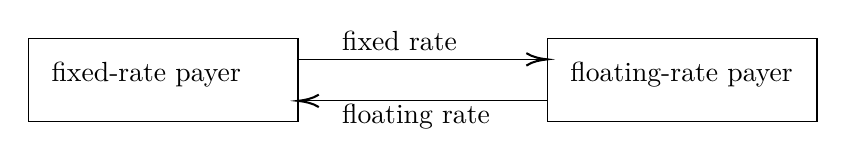
\begin{tikzpicture}[x=0.75pt,y=0.75pt,yscale=-1,xscale=1]

\draw   (0,10) -- (130,10) -- (130,50) -- (0,50) -- cycle ;
\draw    (130,20) -- (250,20) ;
\draw [shift={(250,20)}, rotate = 180] [color={rgb, 255:red, 0; green, 0; blue, 0 }  ][line width=0.75]    (10,-3) .. controls (7,-1) and (3,-0.3) .. (0,0) .. controls (3,0.3) and (7,1) .. (10,3)   ;
\draw    (250,40) -- (130,40) ;
\draw [shift={(130,40)}, rotate = 0] [color={rgb, 255:red, 0; green, 0; blue, 0 }  ][line width=0.75]    (10,-3) .. controls (7,-1) and (3,-0.3) .. (0,0) .. controls (3,0.3) and (7,1) .. (10,3)   ;
\draw   (250,10) -- (380,10) -- (380,50) -- (250,50) -- cycle ;

\draw (10,20) node [anchor=north west][inner sep=0.75pt]   [align=left] {fixed-rate payer};
\draw (150,5) node [anchor=north west][inner sep=0.75pt]   [align=left] {fixed rate};
\draw (150,40) node [anchor=north west][inner sep=0.75pt]   [align=left] {floating rate};
\draw (260,20) node [anchor=north west][inner sep=0.75pt]   [align=left] {floating-rate payer};

\end{tikzpicture}
\end{block}
\end{frame}

\begin{frame}
\begin{block}{Overnight indexed swap}
\protect\hypertarget{overnight-indexed-swap}{}
Interest rate swap wherein a fixed rate of interest (the OIS rate) is
exchanged for a reference rate of interest calculated from a realized
overnight rate (e.g.~SONIA, SOFR).

\begin{itemize}
\tightlist
\item
  If there is only one exchange, the OIS rate is a \textbf{risk-free
  zero rate} equivalent to the UL overnight rate.
\item
  Otherwise, the OIS rates define a risk-free bond worth par.
\item
  An OIS rate can be contrasted with a LIBOR swap, wherein the LIBOR
  rate for a period is known as the start of the period, so the floating
  rate of the first exchange is known.
\end{itemize}
\end{block}
\end{frame}

\begin{frame}{Interest rate swaps: transferring liabilities}
\protect\hypertarget{interest-rate-swaps-transferring-liabilities}{}
Apple uses a swap to convert \textbf{floating}-rate borrowings to
\textbf{fixed}-rate borrowings:

\tikzset{every picture/.style={line width=0.75pt}}

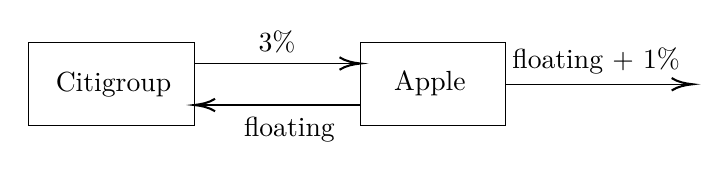
\begin{tikzpicture}[x=0.75pt,y=0.75pt,yscale=-1,xscale=1]

\draw   (0,10) -- (80,10) -- (80,50) -- (0,50) -- cycle ;
\draw    (80,20) -- (160,20) ;
\draw [shift={(160,20)}, rotate = 180] [color={rgb, 255:red, 0; green, 0; blue, 0 }  ][line width=0.75]    (10,-3) .. controls (7,-1) and (3,-0.3) .. (0,0) .. controls (3,0.3) and (7,1) .. (10,3)   ;
\draw    (160,40) -- (80,40) ;
\draw [shift={(80,40)}, rotate = 0] [color={rgb, 255:red, 0; green, 0; blue, 0 }  ][line width=0.75]    (10,-3) .. controls (7,-1) and (3,-0.3) .. (0,0) .. controls (3,0.3) and (7,1) .. (10,3)   ;
\draw   (160,10) -- (230,10) -- (230,50) -- (160,50) -- cycle ;
\draw    (230,30) -- (320,30) ;
\draw [shift={(320,30)}, rotate = 180] [color={rgb, 255:red, 0; green, 0; blue, 0 }  ][line width=0.75]    (10,-3) .. controls (7,-1) and (3,-0.3) .. (0,0) .. controls (3,0.3) and (7,1) .. (10,3)   ;

\draw (12,22.9) node [anchor=north west][inner sep=0.75pt]   [align=left] {Citigroup};
\draw (109.7,3) node [anchor=north west][inner sep=0.75pt]   [align=left] {3\%};
\draw (102.7,44.33) node [anchor=north west][inner sep=0.75pt]   [align=left] {floating};
\draw (175.03,22.23) node [anchor=north west][inner sep=0.75pt]   [align=left] {Apple};
\draw (232,11.07) node [anchor=north west][inner sep=0.75pt]   [align=left] {floating + 1\%};

\end{tikzpicture}

Intel uses a swap to convert \textbf{fixed}-rate borrowings to
\textbf{floating}-rate borrowings:

\tikzset{every picture/.style={line width=0.75pt}}

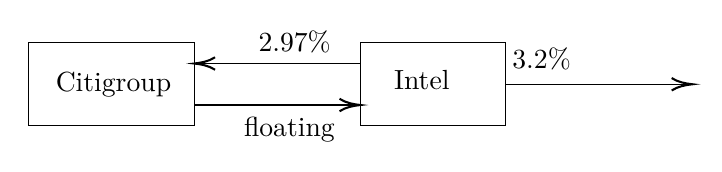
\begin{tikzpicture}[x=0.75pt,y=0.75pt,yscale=-1,xscale=1]

\draw   (0,10) -- (80,10) -- (80,50) -- (0,50) -- cycle ;
\draw    (80,20) -- (160,20) ;
\draw [shift={(80,20)}, rotate = 0] [color={rgb, 255:red, 0; green, 0; blue, 0 }  ][line width=0.75]    (10,-3) .. controls (7,-1) and (3,-0.3) .. (0,0) .. controls (3,0.3) and (7,1) .. (10,3)   ;
\draw    (160,40) -- (80,40) ;
\draw [shift={(160,40)}, rotate = 180] [color={rgb, 255:red, 0; green, 0; blue, 0 }  ][line width=0.75]    (10,-3) .. controls (7,-1) and (3,-0.3) .. (0,0) .. controls (3,0.3) and (7,1) .. (10,3)   ;
\draw   (160,10) -- (230,10) -- (230,50) -- (160,50) -- cycle ;
\draw    (230,30) -- (320,30) ;
\draw [shift={(320,30)}, rotate = 180] [color={rgb, 255:red, 0; green, 0; blue, 0 }  ][line width=0.75]    (10,-3) .. controls (7,-1) and (3,-0.3) .. (0,0) .. controls (3,0.3) and (7,1) .. (10,3)   ;

\draw (12,22.9) node [anchor=north west][inner sep=0.75pt]   [align=left] {Citigroup};
\draw (109.7,3) node [anchor=north west][inner sep=0.75pt]   [align=left] {2.97\%};
\draw (102.7,44.33) node [anchor=north west][inner sep=0.75pt]   [align=left] {floating};
\draw (175.03,22.23) node [anchor=north west][inner sep=0.75pt]   [align=left] {Intel};
\draw (232,11.07) node [anchor=north west][inner sep=0.75pt]   [align=left] {3.2\%};

\end{tikzpicture}
\end{frame}

\begin{frame}{Interest rate swaps: transferring assets}
\protect\hypertarget{interest-rate-swaps-transferring-assets}{}
Apple converts a \textbf{fixed}-rate investment to
\textbf{floating}-rate investment:

\tikzset{every picture/.style={line width=0.75pt}}

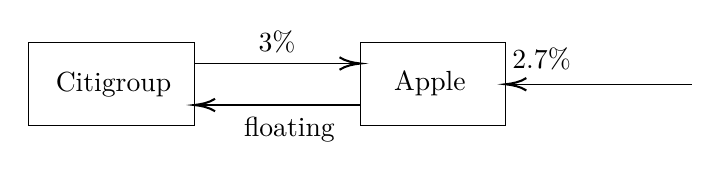
\begin{tikzpicture}[x=0.75pt,y=0.75pt,yscale=-1,xscale=1]

\draw   (0,10) -- (80,10) -- (80,50) -- (0,50) -- cycle ;
\draw    (80,20) -- (160,20) ;
\draw [shift={(160,20)}, rotate = 180] [color={rgb, 255:red, 0; green, 0; blue, 0 }  ][line width=0.75]    (10,-3) .. controls (7,-1) and (3,-0.3) .. (0,0) .. controls (3,0.3) and (7,1) .. (10,3)   ;
\draw    (160,40) -- (80,40) ;
\draw [shift={(80,40)}, rotate = 0] [color={rgb, 255:red, 0; green, 0; blue, 0 }  ][line width=0.75]    (10,-3) .. controls (7,-1) and (3,-0.3) .. (0,0) .. controls (3,0.3) and (7,1) .. (10,3)   ;
\draw   (160,10) -- (230,10) -- (230,50) -- (160,50) -- cycle ;
\draw    (230,30) -- (320,30) ;
\draw [shift={(230,30)}, rotate = 0] [color={rgb, 255:red, 0; green, 0; blue, 0 }  ][line width=0.75]    (10,-3) .. controls (7,-1) and (3,-0.3) .. (0,0) .. controls (3,0.3) and (7,1) .. (10,3)   ;

\draw (12,22.9) node [anchor=north west][inner sep=0.75pt]   [align=left] {Citigroup};
\draw (109.7,3) node [anchor=north west][inner sep=0.75pt]   [align=left] {3\%};
\draw (102.7,44.33) node [anchor=north west][inner sep=0.75pt]   [align=left] {floating};
\draw (175.03,22.23) node [anchor=north west][inner sep=0.75pt]   [align=left] {Apple};
\draw (232,11.07) node [anchor=north west][inner sep=0.75pt]   [align=left] {2.7\%};

\end{tikzpicture}

Intel converts a \textbf{floating}-rate investment to
\textbf{fixed}-rate investment:

\tikzset{every picture/.style={line width=0.75pt}}

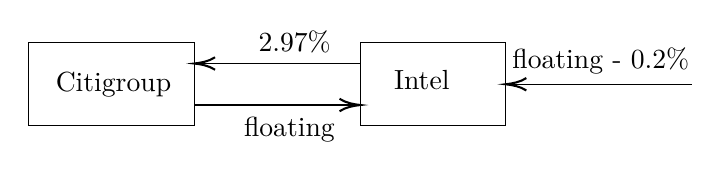
\begin{tikzpicture}[x=0.75pt,y=0.75pt,yscale=-1,xscale=1]

\draw   (0,10) -- (80,10) -- (80,50) -- (0,50) -- cycle ;
\draw    (80,20) -- (160,20) ;
\draw [shift={(80,20)}, rotate = 0] [color={rgb, 255:red, 0; green, 0; blue, 0 }  ][line width=0.75]    (10,-3) .. controls (7,-1) and (3,-0.3) .. (0,0) .. controls (3,0.3) and (7,1) .. (10,3)   ;
\draw    (160,40) -- (80,40) ;
\draw [shift={(160,40)}, rotate = 180] [color={rgb, 255:red, 0; green, 0; blue, 0 }  ][line width=0.75]    (10,-3) .. controls (7,-1) and (3,-0.3) .. (0,0) .. controls (3,0.3) and (7,1) .. (10,3)   ;
\draw   (160,10) -- (230,10) -- (230,50) -- (160,50) -- cycle ;
\draw    (230,30) -- (320,30) ;
\draw [shift={(230,30)}, rotate = 0] [color={rgb, 255:red, 0; green, 0; blue, 0 }  ][line width=0.75]    (10,-3) .. controls (7,-1) and (3,-0.3) .. (0,0) .. controls (3,0.3) and (7,1) .. (10,3)   ;

\draw (12,22.9) node [anchor=north west][inner sep=0.75pt]   [align=left] {Citigroup};
\draw (109.7,3) node [anchor=north west][inner sep=0.75pt]   [align=left] {2.97\%};
\draw (102.7,44.33) node [anchor=north west][inner sep=0.75pt]   [align=left] {floating};
\draw (175.03,22.23) node [anchor=north west][inner sep=0.75pt]   [align=left] {Intel};
\draw (232,11.07) node [anchor=north west][inner sep=0.75pt]   [align=left] {floating - 0.2\%};

\end{tikzpicture}
\end{frame}

\begin{frame}{Comparative advantage}
\protect\hypertarget{comparative-advantage}{}
Why use swaps? One reason might be \textbf{comparative advantage}: a
company might have a relative advantage to borrowing in either
fixed-rate markets or floating-rate markets.

\begin{longtable}[]{@{}lll@{}}
\toprule
& fixed rate & floating rate \\
\midrule
\endhead
AAACorp & 4.0\% & floating - 0.1\% \\
BBBCorp & 5.2\% & floating + 0.6\% \\
\bottomrule
\end{longtable}

Here, AAACorp and BBBCorp might seek to collaborate:

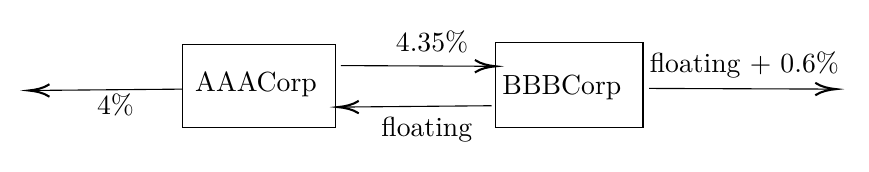
\begin{tikzpicture}[x=0.75pt,y=0.75pt,yscale=-1,xscale=1]

\draw   (75,10) -- (149,10) -- (149,50) -- (75,50) -- cycle ;
\draw    (151.37,20) -- (224,20.33) ;
\draw [shift={(226,20.34)}, rotate = 180.26] [color={rgb, 255:red, 0; green, 0; blue, 0 }  ][line width=0.75]    (10,-3) .. controls (7,-1) and (3.31,-0.3) .. (0,0) .. controls (3.31,0.3) and (7,1) .. (10,3)   ;
\draw    (224,39.34) -- (152.03,39.98) ;
\draw [shift={(150.03,40)}, rotate = 0] [color={rgb, 255:red, 0; green, 0; blue, 0 }  ][line width=0.75]    (10,-3) .. controls (7,-1) and (3.31,-0.3) .. (0,0) .. controls (3.31,0.3) and (7,1) .. (10,3)   ;
\draw   (225.73,9.07) -- (297,9.07) -- (297,50) -- (225.73,50) -- cycle ;
\draw    (300,31) -- (388,31.33) ;
\draw [shift={(390,31.34)}, rotate = 180.21] [color={rgb, 255:red, 0; green, 0; blue, 0 }  ][line width=0.75]    (10,-3) .. controls (7,-1) and (3.31,-0.3) .. (0,0) .. controls (3.31,0.3) and (7,1) .. (10,3)   ;
\draw    (75,31.34) -- (3.03,31.98) ;
\draw [shift={(1.03,32)}, rotate = 0] [color={rgb, 255:red, 0; green, 0; blue, 0 }  ][line width=0.75]    (10,-3) .. controls (7,-1) and (3.31,-0.3) .. (0,0) .. controls (3.31,0.3) and (7,1) .. (10,3)   ;

\draw (80,21.9) node [anchor=north west][inner sep=0.75pt]   [align=left] {AAACorp};
\draw (176.7,2) node [anchor=north west][inner sep=0.75pt]   [align=left] {4.35\%};
\draw (169.7,43.33) node [anchor=north west][inner sep=0.75pt]   [align=left] {floating};
\draw (228,23.34) node [anchor=north west][inner sep=0.75pt]   [align=left] {BBBCorp};
\draw (299,12.07) node [anchor=north west][inner sep=0.75pt]   [align=left] {floating + 0.6\%};
\draw (32.7,32.33) node [anchor=north west][inner sep=0.75pt]   [align=left] {4\%};


\end{tikzpicture}
\end{frame}

\begin{frame}
In practice, the swap might be \textbf{brokered} by a financial
institution:

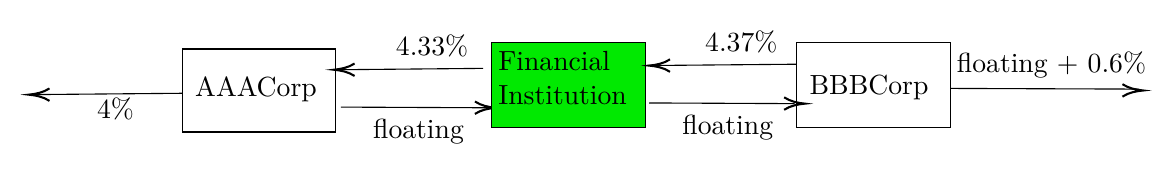
\begin{tikzpicture}[x=0.75pt,y=0.75pt,yscale=-1,xscale=1]

\draw   (75,10) -- (149,10) -- (149,50) -- (75,50) -- cycle ;
\draw    (151.37,38) -- (224,38.33) ;
\draw [shift={(226,38.34)}, rotate = 180.26] [color={rgb, 255:red, 0; green, 0; blue, 0 }  ][line width=0.75]    (10,-3) .. controls (7,-1) and (3.31,-0.3) .. (0,0) .. controls (3.31,0.3) and (7,1) .. (10,3)   ;
\draw    (220,19.34) -- (150.03,20) ;
\draw [shift={(148.03,20)}, rotate = 0] [color={rgb, 255:red, 0; green, 0; blue, 0 }  ][line width=0.75]    (10,-3) .. controls (7,-1) and (3.31,-0.3) .. (0,0) .. controls (3.31,0.3) and (7,1) .. (10,3)   ;
\draw   (370.73,7.07) -- (445,7.07) -- (445,48) -- (370.73,48) -- cycle ;
\draw    (445.37,29) -- (505,29.22) -- (536,29.33) ;
\draw [shift={(538,30)}, rotate = 180.21] [color={rgb, 255:red, 0; green, 0; blue, 0 }  ][line width=0.75]    (10,-3) .. controls (7,-1) and (3.31,-0.3) .. (0,0) .. controls (3.31,0.3) and (7,1) .. (10,3)   ;
\draw    (75,31.34) -- (3.03,31.98) ;
\draw [shift={(1.03,32)}, rotate = 0] [color={rgb, 255:red, 0; green, 0; blue, 0 }  ][line width=0.75]    (10,-3) .. controls (7,-1) and (3.31,-0.3) .. (0,0) .. controls (3.31,0.3) and (7,1) .. (10,3)   ;
\draw  [fill={rgb, 255:red, 1; green, 233; blue, 1 }  ,fill opacity=1 ] (224,6.73) -- (298,6.73) -- (298,47.67) -- (224,47.67) -- cycle ;
\draw    (300,36) -- (370,36.33) ;
\draw [shift={(375,36.34)}, rotate = 180.26] [color={rgb, 255:red, 0; green, 0; blue, 0 }  ][line width=0.75]    (10,-3) .. controls (7,-1) and (3.31,-0.3) .. (0,0) .. controls (3.31,0.3) and (7,1) .. (10,3)   ;
\draw    (371,17.34) -- (299.03,17.98) ;
\draw [shift={(300,18)}, rotate = 0] [color={rgb, 255:red, 0; green, 0; blue, 0 }  ][line width=0.75]    (10,-3) .. controls (7,-1) and (3.31,-0.3) .. (0,0) .. controls (3.31,0.3) and (7,1) .. (10,3)   ;

\draw (80,21.9) node [anchor=north west][inner sep=0.75pt]   [align=left] {AAACorp};
\draw (176.7,2) node [anchor=north west][inner sep=0.75pt]   [align=left] {4.33\%};
\draw (165.7,42.33) node [anchor=north west][inner sep=0.75pt]   [align=left] {floating};
\draw (376,21.34) node [anchor=north west][inner sep=0.75pt]   [align=left] {BBBCorp};
\draw (447,10.07) node [anchor=north west][inner sep=0.75pt]   [align=left] {floating + 0.6\%};
\draw (32.7,32.33) node [anchor=north west][inner sep=0.75pt]   [align=left] {4\%};
\draw (226,10) node [anchor=north west][inner sep=0.75pt]   [align=left] {Financial\\Institution};
\draw (325.7,0) node [anchor=north west][inner sep=0.75pt]   [align=left] {4.37\%};
\draw (314.7,40.33) node [anchor=north west][inner sep=0.75pt]   [align=left] {floating};


\end{tikzpicture}

Why has comparative advantage not been arbitraged away?

The \textbf{maturities} of contracts available via fixed-rate financing
are generally different than those available via floating-rate
financing:

\begin{itemize}
\tightlist
\item
  Fixed-rate contracts are often longer than floating-rate contracts
\item
  The spread over the reference rate can effectively be adjusted by
  floating-rate lenders
\item
  Fixed-rate lenders often lack this option
\end{itemize}
\end{frame}

\begin{frame}{Currency swaps}
\protect\hypertarget{currency-swaps}{}
\textbf{fixed-for-fixed currency swap}: arrangement wherein principal
and interest payments in one currency are exchanged for principal and
interest payments in another currency

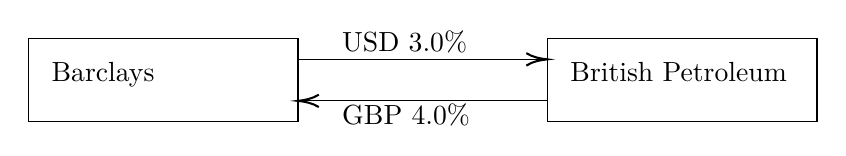
\begin{tikzpicture}[x=0.75pt,y=0.75pt,yscale=-1,xscale=1]

\draw   (0,10) -- (130,10) -- (130,50) -- (0,50) -- cycle ;
\draw    (130,20) -- (250,20) ;
\draw [shift={(250,20)}, rotate = 180] [color={rgb, 255:red, 0; green, 0; blue, 0 }  ][line width=0.75]    (10,-3) .. controls (7,-1) and (3,-0.3) .. (0,0) .. controls (3,0.3) and (7,1) .. (10,3)   ;
\draw    (250,40) -- (130,40) ;
\draw [shift={(130,40)}, rotate = 0] [color={rgb, 255:red, 0; green, 0; blue, 0 }  ][line width=0.75]    (10,-3) .. controls (7,-1) and (3,-0.3) .. (0,0) .. controls (3,0.3) and (7,1) .. (10,3)   ;
\draw   (250,10) -- (380,10) -- (380,50) -- (250,50) -- cycle ;

\draw (10,20) node [anchor=north west][inner sep=0.75pt]   [align=left] {Barclays};
\draw (150,5) node [anchor=north west][inner sep=0.75pt]   [align=left] {USD 3.0\%};
\draw (150,40) node [anchor=north west][inner sep=0.75pt]   [align=left] {GBP 4.0\%};
\draw (260,20) node [anchor=north west][inner sep=0.75pt]   [align=left] {British Petroleum};

\end{tikzpicture}

Variations:

\begin{itemize}
\tightlist
\item
  fixed-for-floating currency swap
\item
  floating-for-floating currency swap
\item
  quanto (or diff swap): arrangement wherein a rate observed in one
  currency is applied to a principal amount in another currency
\end{itemize}
\end{frame}

\begin{frame}[shrink]{Currency swaps: example with comparative
advantage}
\protect\hypertarget{currency-swaps-example-with-comparative-advantage}{}
Suppose that General Electric has a \textbf{comparative advantage} to
borrowing in USD and Qantas Airways has a \textbf{comparative advantage}
to borrowing in AUD. Financial institution could reduce both of their
costs by taking on FX risk:

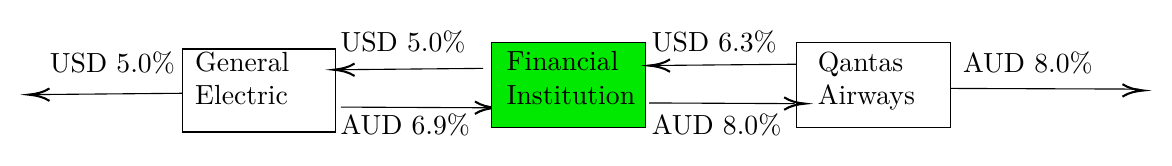
\begin{tikzpicture}[x=0.75pt,y=0.75pt,yscale=-1,xscale=1]

\draw   (75,10) -- (149,10) -- (149,50) -- (75,50) -- cycle ;
\draw    (151.37,38) -- (224,38.33) ;
\draw [shift={(226,38.34)}, rotate = 180.26] [color={rgb, 255:red, 0; green, 0; blue, 0 }  ][line width=0.75]    (10,-3) .. controls (7,-1) and (3.31,-0.3) .. (0,0) .. controls (3.31,0.3) and (7,1) .. (10,3)   ;
\draw    (220,19.34) -- (150.03,20) ;
\draw [shift={(148.03,20)}, rotate = 0] [color={rgb, 255:red, 0; green, 0; blue, 0 }  ][line width=0.75]    (10,-3) .. controls (7,-1) and (3.31,-0.3) .. (0,0) .. controls (3.31,0.3) and (7,1) .. (10,3)   ;
\draw   (370.73,7.07) -- (445,7.07) -- (445,48) -- (370.73,48) -- cycle ;
\draw    (445.37,29) -- (505,29.22) -- (536,29.33) ;
\draw [shift={(538,30)}, rotate = 180.21] [color={rgb, 255:red, 0; green, 0; blue, 0 }  ][line width=0.75]    (10,-3) .. controls (7,-1) and (3.31,-0.3) .. (0,0) .. controls (3.31,0.3) and (7,1) .. (10,3)   ;
\draw    (75,31.34) -- (3.03,31.98) ;
\draw [shift={(1.03,32)}, rotate = 0] [color={rgb, 255:red, 0; green, 0; blue, 0 }  ][line width=0.75]    (10,-3) .. controls (7,-1) and (3.31,-0.3) .. (0,0) .. controls (3.31,0.3) and (7,1) .. (10,3)   ;
\draw  [fill={rgb, 255:red, 1; green, 233; blue, 1 }  ,fill opacity=1 ] (224,6.73) -- (298,6.73) -- (298,47.67) -- (224,47.67) -- cycle ;
\draw    (300,36) -- (370,36.33) ;
\draw [shift={(375,36.34)}, rotate = 180.26] [color={rgb, 255:red, 0; green, 0; blue, 0 }  ][line width=0.75]    (10,-3) .. controls (7,-1) and (3.31,-0.3) .. (0,0) .. controls (3.31,0.3) and (7,1) .. (10,3)   ;
\draw    (371,17.34) -- (299.03,17.98) ;
\draw [shift={(300,18)}, rotate = 0] [color={rgb, 255:red, 0; green, 0; blue, 0 }  ][line width=0.75]    (10,-3) .. controls (7,-1) and (3.31,-0.3) .. (0,0) .. controls (3.31,0.3) and (7,1) .. (10,3)   ;

\draw (80,10) node [anchor=north west][inner sep=0.75pt]   [align=left] {General\\Electric};
\draw (380,10) node [anchor=north west][inner sep=0.75pt]   [align=left] {Qantas\\Airways};
\draw (230,10) node [anchor=north west][inner sep=0.75pt]   [align=left] {Financial\\Institution};

\draw (10,10) node [anchor=north west][inner sep=0.75pt]   [align=left] {USD 5.0\%};

\draw (150,0) node [anchor=north west][inner sep=0.75pt]   [align=left] {USD 5.0\%};
\draw (150,40) node [anchor=north west][inner sep=0.75pt]   [align=left] {AUD 6.9\%};

\draw (300,0) node [anchor=north west][inner sep=0.75pt]   [align=left] {USD 6.3\%};
\draw (300,40) node [anchor=north west][inner sep=0.75pt]   [align=left] {AUD 8.0\%};

\draw (450,10) node [anchor=north west][inner sep=0.75pt]   [align=left] {AUD 8.0\%};

\end{tikzpicture}

It might be more cost-effective for Quantas Airways to bear some FX
risk:

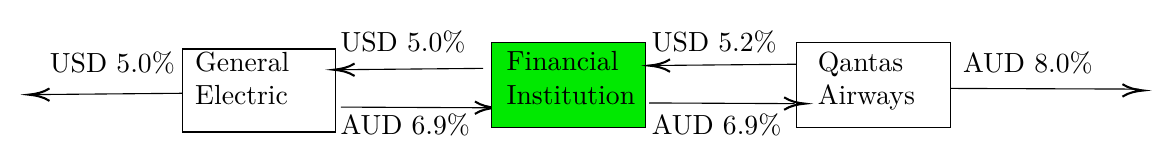
\begin{tikzpicture}[x=0.75pt,y=0.75pt,yscale=-1,xscale=1]

\draw   (75,10) -- (149,10) -- (149,50) -- (75,50) -- cycle ;
\draw    (151.37,38) -- (224,38.33) ;
\draw [shift={(226,38.34)}, rotate = 180.26] [color={rgb, 255:red, 0; green, 0; blue, 0 }  ][line width=0.75]    (10,-3) .. controls (7,-1) and (3.31,-0.3) .. (0,0) .. controls (3.31,0.3) and (7,1) .. (10,3)   ;
\draw    (220,19.34) -- (150.03,20) ;
\draw [shift={(148.03,20)}, rotate = 0] [color={rgb, 255:red, 0; green, 0; blue, 0 }  ][line width=0.75]    (10,-3) .. controls (7,-1) and (3.31,-0.3) .. (0,0) .. controls (3.31,0.3) and (7,1) .. (10,3)   ;
\draw   (370.73,7.07) -- (445,7.07) -- (445,48) -- (370.73,48) -- cycle ;
\draw    (445.37,29) -- (505,29.22) -- (536,29.33) ;
\draw [shift={(538,30)}, rotate = 180.21] [color={rgb, 255:red, 0; green, 0; blue, 0 }  ][line width=0.75]    (10,-3) .. controls (7,-1) and (3.31,-0.3) .. (0,0) .. controls (3.31,0.3) and (7,1) .. (10,3)   ;
\draw    (75,31.34) -- (3.03,31.98) ;
\draw [shift={(1.03,32)}, rotate = 0] [color={rgb, 255:red, 0; green, 0; blue, 0 }  ][line width=0.75]    (10,-3) .. controls (7,-1) and (3.31,-0.3) .. (0,0) .. controls (3.31,0.3) and (7,1) .. (10,3)   ;
\draw  [fill={rgb, 255:red, 1; green, 233; blue, 1 }  ,fill opacity=1 ] (224,6.73) -- (298,6.73) -- (298,47.67) -- (224,47.67) -- cycle ;
\draw    (300,36) -- (370,36.33) ;
\draw [shift={(375,36.34)}, rotate = 180.26] [color={rgb, 255:red, 0; green, 0; blue, 0 }  ][line width=0.75]    (10,-3) .. controls (7,-1) and (3.31,-0.3) .. (0,0) .. controls (3.31,0.3) and (7,1) .. (10,3)   ;
\draw    (371,17.34) -- (299.03,17.98) ;
\draw [shift={(300,18)}, rotate = 0] [color={rgb, 255:red, 0; green, 0; blue, 0 }  ][line width=0.75]    (10,-3) .. controls (7,-1) and (3.31,-0.3) .. (0,0) .. controls (3.31,0.3) and (7,1) .. (10,3)   ;

\draw (80,10) node [anchor=north west][inner sep=0.75pt]   [align=left] {General\\Electric};
\draw (380,10) node [anchor=north west][inner sep=0.75pt]   [align=left] {Qantas\\Airways};
\draw (230,10) node [anchor=north west][inner sep=0.75pt]   [align=left] {Financial\\Institution};

\draw (10,10) node [anchor=north west][inner sep=0.75pt]   [align=left] {USD 5.0\%};

\draw (150,0) node [anchor=north west][inner sep=0.75pt]   [align=left] {USD 5.0\%};
\draw (150,40) node [anchor=north west][inner sep=0.75pt]   [align=left] {AUD 6.9\%};

\draw (300,0) node [anchor=north west][inner sep=0.75pt]   [align=left] {USD 5.2\%};
\draw (300,40) node [anchor=north west][inner sep=0.75pt]   [align=left] {AUD 6.9\%};

\draw (450,10) node [anchor=north west][inner sep=0.75pt]   [align=left] {AUD 8.0\%};

\end{tikzpicture}

Or it might be more cost-effective for General Electric to bear some FX
risk:

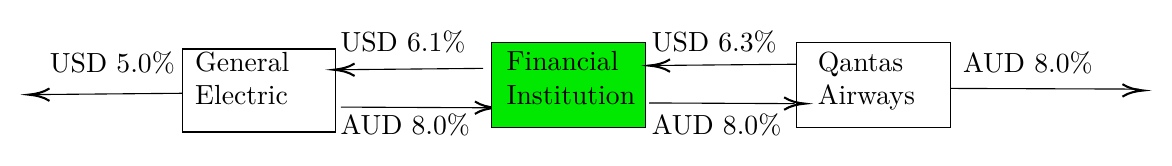
\begin{tikzpicture}[x=0.75pt,y=0.75pt,yscale=-1,xscale=1]

\draw   (75,10) -- (149,10) -- (149,50) -- (75,50) -- cycle ;
\draw    (151.37,38) -- (224,38.33) ;
\draw [shift={(226,38.34)}, rotate = 180.26] [color={rgb, 255:red, 0; green, 0; blue, 0 }  ][line width=0.75]    (10,-3) .. controls (7,-1) and (3.31,-0.3) .. (0,0) .. controls (3.31,0.3) and (7,1) .. (10,3)   ;
\draw    (220,19.34) -- (150.03,20) ;
\draw [shift={(148.03,20)}, rotate = 0] [color={rgb, 255:red, 0; green, 0; blue, 0 }  ][line width=0.75]    (10,-3) .. controls (7,-1) and (3.31,-0.3) .. (0,0) .. controls (3.31,0.3) and (7,1) .. (10,3)   ;
\draw   (370.73,7.07) -- (445,7.07) -- (445,48) -- (370.73,48) -- cycle ;
\draw    (445.37,29) -- (505,29.22) -- (536,29.33) ;
\draw [shift={(538,30)}, rotate = 180.21] [color={rgb, 255:red, 0; green, 0; blue, 0 }  ][line width=0.75]    (10,-3) .. controls (7,-1) and (3.31,-0.3) .. (0,0) .. controls (3.31,0.3) and (7,1) .. (10,3)   ;
\draw    (75,31.34) -- (3.03,31.98) ;
\draw [shift={(1.03,32)}, rotate = 0] [color={rgb, 255:red, 0; green, 0; blue, 0 }  ][line width=0.75]    (10,-3) .. controls (7,-1) and (3.31,-0.3) .. (0,0) .. controls (3.31,0.3) and (7,1) .. (10,3)   ;
\draw  [fill={rgb, 255:red, 1; green, 233; blue, 1 }  ,fill opacity=1 ] (224,6.73) -- (298,6.73) -- (298,47.67) -- (224,47.67) -- cycle ;
\draw    (300,36) -- (370,36.33) ;
\draw [shift={(375,36.34)}, rotate = 180.26] [color={rgb, 255:red, 0; green, 0; blue, 0 }  ][line width=0.75]    (10,-3) .. controls (7,-1) and (3.31,-0.3) .. (0,0) .. controls (3.31,0.3) and (7,1) .. (10,3)   ;
\draw    (371,17.34) -- (299.03,17.98) ;
\draw [shift={(300,18)}, rotate = 0] [color={rgb, 255:red, 0; green, 0; blue, 0 }  ][line width=0.75]    (10,-3) .. controls (7,-1) and (3.31,-0.3) .. (0,0) .. controls (3.31,0.3) and (7,1) .. (10,3)   ;

\draw (80,10) node [anchor=north west][inner sep=0.75pt]   [align=left] {General\\Electric};
\draw (380,10) node [anchor=north west][inner sep=0.75pt]   [align=left] {Qantas\\Airways};
\draw (230,10) node [anchor=north west][inner sep=0.75pt]   [align=left] {Financial\\Institution};

\draw (10,10) node [anchor=north west][inner sep=0.75pt]   [align=left] {USD 5.0\%};

\draw (150,0) node [anchor=north west][inner sep=0.75pt]   [align=left] {USD 6.1\%};
\draw (150,40) node [anchor=north west][inner sep=0.75pt]   [align=left] {AUD 8.0\%};

\draw (300,0) node [anchor=north west][inner sep=0.75pt]   [align=left] {USD 6.3\%};
\draw (300,40) node [anchor=north west][inner sep=0.75pt]   [align=left] {AUD 8.0\%};

\draw (450,10) node [anchor=north west][inner sep=0.75pt]   [align=left] {AUD 8.0\%};

\end{tikzpicture}
\end{frame}

\begin{frame}{Other swaps}
\protect\hypertarget{other-swaps}{}
\textbf{Equity swap}: agreement to exchange the total return (dividends
plus gains) of an equity index for a fixed for floating rate of
interest.

\textbf{Credit default swap}: agreement that generates a payment if a
particular company (the reference entity) defaults

\begin{itemize}
\tightlist
\item
  the \textbf{protection buyer} pays the \textbf{CDS spread} (and
  insurance premium) over the life of the contract
\item
  in the event of default, the \textbf{protection seller} pays an amount
  that would restore the value of the hypothetical portfolio of the
  bonds of the reference entity to the value of its principal
\end{itemize}

Options:

\begin{itemize}
\tightlist
\item
  entendable swap: one party can extend the swap arrangement
\item
  puttable swap: one party can terminate the swap arrangement early
\item
  swaption: option on a swap
\end{itemize}
\end{frame}

\begin{frame}{Thank you!}
\protect\hypertarget{thank-you}{}
\textbf{Contact}

\vspace{0.6cm}

Jiahua (Java) Xu

\vspace{0.4cm}

UCL Centre for Blockchain Technologies

66-72 Gower Street

\vspace{0.4cm}

\href{mailto:jiahua.xu@ucl.ac.uk}{\nolinkurl{jiahua.xu@ucl.ac.uk}}
\end{frame}

\begin{frame}[allowframebreaks]{References}
\protect\hypertarget{references}{}
\small

\widowpenalties 1 0
\end{frame}

\end{document}
